\section{Evaluation}
\label{sec:evaluation}

Below, we evaluate the performance of \ac{name} in our prototype implementation.
We first describe the domains represented by the signaling set,
including how we identified these domains. Next, we compare different approaches
and optimizations for representing the signaling set. Finally, we describe the
performance effects of \ac{name} on connection establishment.

\subsection{Signaling Set Domains}
\label{sec:evaluation:https}

Before building a representation of the signaling set, we need to determine
which domains belong in it. Moreover, to determine the long-term
viability of our solution, we also need to understand how the size of this set
of domains may change in the future. Addressing both of these problems requires
a complete and accurate view of the Web \ac{pki}, namely, the set of domains
that are accessible over HTTPS.

We can obtain a view of the Web \ac{pki} using data from public logs (\autoref{sec:design:signaling}). 
Specifically, we obtain public-key
certificates from Censys~\cite{durumeric2015search} and logs in
\ac{ct}~\cite{rfc6962}. From Censys, we collected 1,026 scans of the IPv4
address space from September 12, 2015 to July 3, 2018.
From \ac{ct}, we collected all entries from known \ac{ct} logs that were not
disqualified or unreachable as of July 3,
2018,\footnote{\url{https://www.certificate-transparency.org/known-logs}} which
totaled approximately 1.74B certificates from 26 logs from
March 26, 2013 to July 3, 2018.

%\begin{figure*}
  %\centering
  %\subfloat[Certs.]{
    %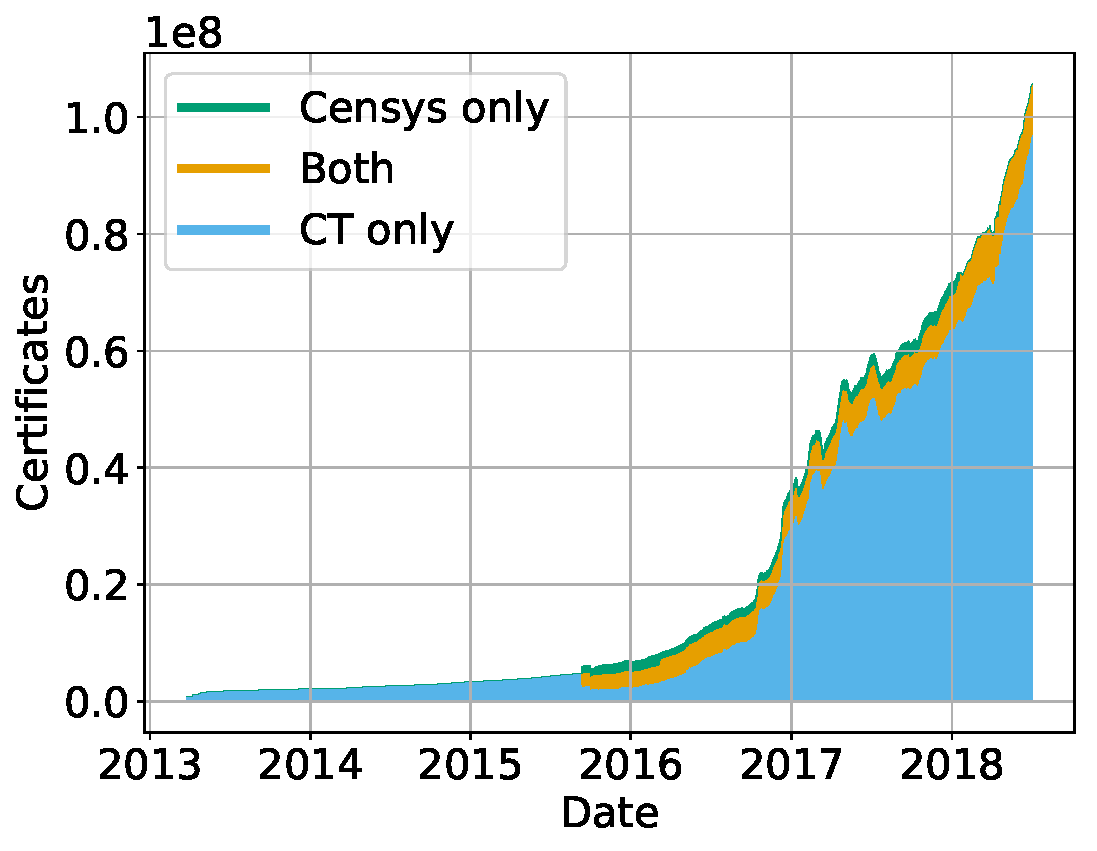
\includegraphics[width=0.5\linewidth]{fig/cert_count_valid}
    %\label{fig:count:certs}
  %}
  %\subfloat[Names.]{
    %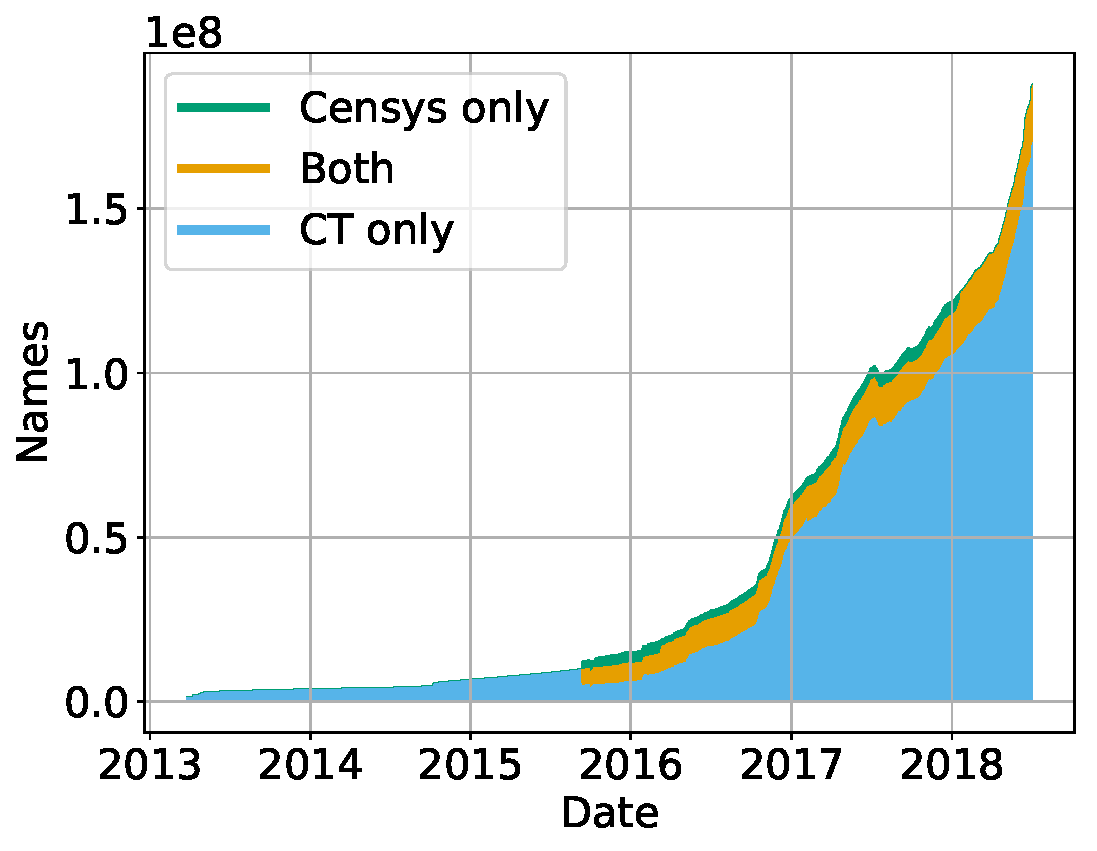
\includegraphics[width=0.5\linewidth]{fig/name_count_valid}
    %\label{fig:count:names}
  %}
  %\caption{Number of unique certificates and domain names in the Web \ac{pki} as seen by
  %Censys and \ac{ct}.}
  %\label{fig:count}
%\end{figure*}

\begin{figure}
  \centering
  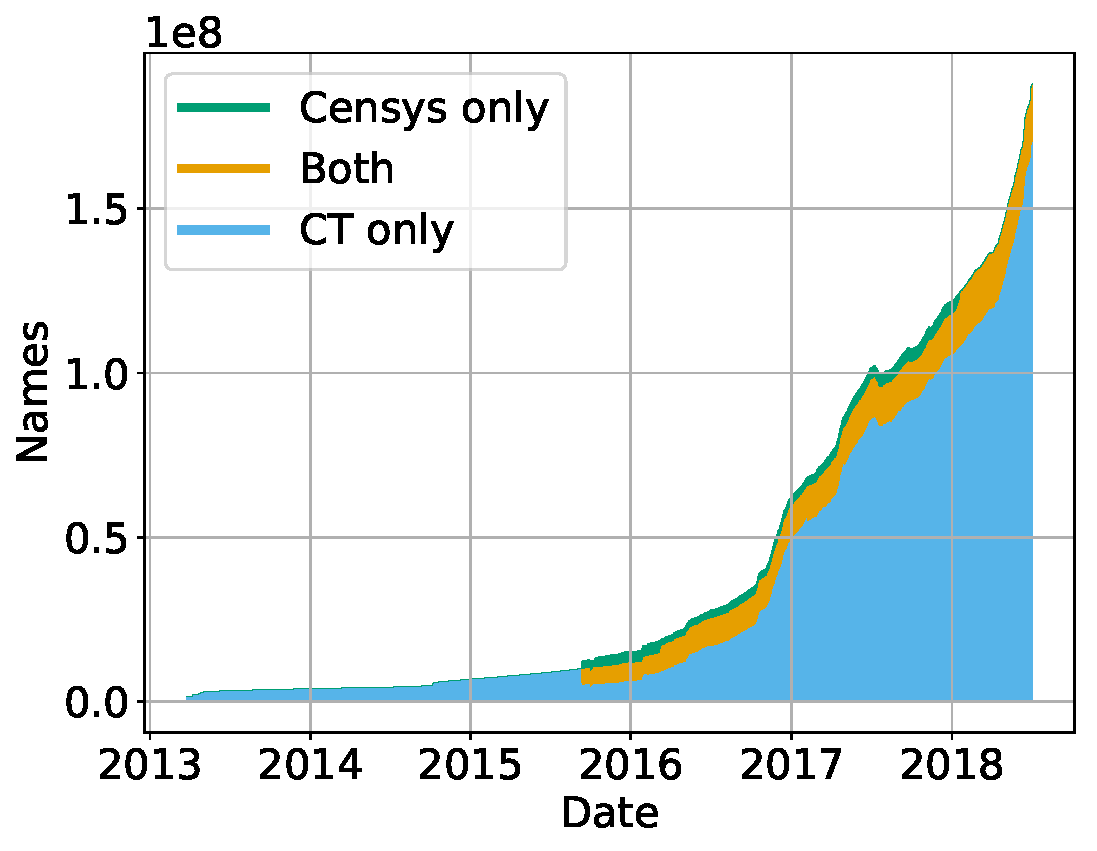
\includegraphics[width=\linewidth]{fig/name_count_valid}
  \label{fig:count:names}
  %\caption{Number of unique certificates and domain names in the Web \ac{pki} as seen by
  %Censys and \ac{ct}.}
  \caption{Number of unique names (including hostnames and wildcard names) seen
  by Censys and \ac{ct} over time.}
  %\label{fig:count}
\end{figure}

On each of these days, we consider an ``active set'' of certificates consisting
of all certificates that were valid on that day and had an associated
certificate chain rooted in one of the three major root certificate stores,
determined by Apple, Microsoft, or Mozilla. In the Censys dataset, because we
observed a great deal of churn (i.e., certificates disappearing and appearing in
consecutive scans), we included a certificate in the active set from the
time it was first observed in our data until its expiration. We then consider
the number of unique, valid domain names, which we use to build the signaling
set.

Figures~\ref{fig:count:certs} and~\ref{fig:count:names} show the number
of domain names observed by Censys, \ac{ct}, and their overlap over time. Our
results show that \ac{ct} observes vastly more certificates (and consequently
names) than Censys. It is unclear what accounts for this large discrepancy. One
possibility is that many certificates are simply never deployed in public-facing
HTTPS sites. Another likely contributing factor is the increasing prevalence of
Server Name Indication (SNI)~\cite{rfc6066}, which would cause Censys' probes to
be rejected when they do not include the correct server name.

From Censys and \ac{ct}, we obtained a total of 156,289,973 valid domain names
for which a certificate had been issued. To address the possibility that many of
these names may not be used for public-facing sites, we performed a scan of port
443 (the default for \ac{https}) using ZGrab~\cite{durumeric2015search} for all
of these domain names, and discarded any domain names that failed to respond.
This resulted in a set of 64,050,329 names that we used for testing, as
described below.

\subsection{Signaling Set Representation}
\label{sec:evaluation:implementation}

As described in \autoref{sec:design:signaling}, our motivation for using
\iac{dafsa}-based representation of the signaling set was twofold: first, the
representation has no false positives or negatives, and second, it can be
searched in its compressed state, leading to a lower memory usage requirement
for clients. To evaluate the effectiveness of these design decisions against
other alternatives, we conducted an experiment to measure the space requirements
for the signaling set in various representations. We measured both the fully
compressed size (which dictates bandwidth usage when transmitting the set to the
client and the client's overhead storing it on disk) and the size in memory
(when being used by the client during certificate verification).

In particular, we compared the plaintext representation of the signaling set (as
of July 3, 2018) with a compressed representation using Bloom filters, the
generic compression utility zpaq~\cite{zpaq},\footnote{While we tested
  compression with other utilities, zpaq had the smallest size. Thus we used
zpaq for the experiment to compare a near-best-case compression scenario.} and
various configurations of our \ac{dafsa}-based representation. We also
compressed the \ac{dafsa}-based representation using zpaq to find its size on
disk and in transit. 

We specifically tested a Bloom filter with false positive rates of 0.001\%,
0.01\%, and 0.1\%. Since the number of domain names is on the order of
100M~\cite{dnib-14-1}, we expect that the number of false positives will be on
the order of 1k, 10k, and 100k, respectively. We estimate that a false positive
rate of 0.001\% will be sufficient for most users. We tested zpaq using two
compression methods, 1 and 5, where method 1 completes in a short amount of time
(25 seconds) but compresses the input less while method 5 takes a long time (20
minutes) but yields excellent compression. Furthermore, with zpaq method 5, we
tested with 64 MiB and 2048 MiB blocks, where larger blocks typically yield
better compression. Finally, with our \ac{dafsa}-based representation, we tested
a plain encoding as well as an encoding using our path-compressed \ac{dafsa},
and compressed each of these encodings with zpaq method 5 using both block
sizes.

\section{Signaling HTTPS Deployment}
\label{sec:signaling}

In this section, we describe the details of how we signal \ac{https} deployment
in \ac{name}.

\subsection{Data Sources}

The authors of CRLite~\cite{larisch2017crlite} observed that
Censys~\cite{durumeric2015search} and Google's set of \ac{ct}
logs\footnote{\url{https://www.certificate-transparency.org/known-logs}} have
played a critical role in making the set of all currently known \ac{tls}
certificates easily accessible. While the authors of CRLite used this knowledge
to space-efficiently store the set of all revoked certificates, in \ac{name} we
are interested in space-efficiently storing the set of all domains that have
deployed \ac{https}. We note that we can use the same data sources as CRLite
does and simply extract the set of domain names appearing in currently valid
certificates to obtain a list of all domains deploying \ac{https}.

To this end, Censys provides a scan of the entire IPv4 address space on port 443
(the default port number for \ac{https}) and the resulting \ac{tls} handshake
attempts.  \steve{(todo) We also downloaded a dump of XX \ac{ct} logs and
extracted domain names from the certificates stored at these logs.} After
extracting the data from the \steve{(update) May 18, 2017} scan results
\steve{(todo) and from the \ac{ct} log databasse}, we obtained a list of
\steve{(update) just over 69 million} domain names that take up a total of
\steve{(update) 147 MB}. This set excludes duplicate domain names as well as
common names \steve{(todo) explain in background} that are invalid DNS names.

\subsection{Approaches}

\steve{This subsection is in note form, and for now is just to summarize the
approaches I have tried.}

CRLite makes use of filter cascades (based on Bloom filters) to efficiently
store the set of all revoked certificates in around 10 MB. However, CRLite's
approach relies on having access to the set of all known certificates, which
Censys and the \ac{ct} logs can provide. While it is possible to access many of
the top-level domain zone files in DNS (including \texttt{.com}), many of the
registrars of country-specific top-level domains do not publicize their
information. Moreover, CRLite relies on the \steve{reasonable} assumption that
only a small minority of certificates will be revoked. By contrast, the rate of
\ac{https} deployment cannot be bounded by such assumptions, particular with the
advent of services such as Let's Encrypt, which has already increased the
\ac{https} deployment rate in its early stages \steve{(todo) wording}.

Constructing the signal set by simply compressing the set of \ac{https} domains
is also possible. As with most data compression algorithms, there is a clear
tradeoff between speed and compression ratio. For example, using lz4
\steve{(todo) cite} takes less than a second to compress and decompress, but
only obtains a compression ratio of 2.26 (for a compressed size of 65 MB). Using
bzip2, on the other hand, takes just over 10 seconds and has a ratio of 3.68 (40
MB compressed). Using xz took 64 seconds and produced a ratio of 4.45 (33 MB
compressed), and the best performer, zpaq (with the largest block size), took
4.5 minutes and produced a ratio of 5.88 (25 MB compressed). Unfortunately,
decompression with zpaq is slow, taking 7 minutes, and thus cannot be used to
support real-time signal set checking.

Succinct data structures provide a way for us to encode the signal set in a
space-efficient way while supporting efficient membership queries in the
succinctly encoded state. If we build a trie (also called a prefix tree) based
on the reversed domain names (capturing the highly repeated use of TLDs), we can
use the LOUDS (level order unary degree sequence) representation of the prefix
tree to efficiently encode the tree. In particular, we can represent the full
signal set in 73.3 MB. \steve{We also tried the use of minimal acyclic finite
  state automata (MAFSAs), which can represent the same information as a trie in
fewer states. However, this approach is quite slow for the number of domains we
want to represent, and there are fewer ways of efficiently encoding MAFSAs,
which in our case are effectively directed acyclic graphs with labeled edges.}

\subsection{Client Procedure}

\steve{How the client actually performs the lookup}


\begin{table}[tbp]
  \centering
  \caption{Size (on-disk or in transit) of \ac{name} signaling set on
    July 3, 2018 (\numnames{} names) with various compression approaches. The
    representation size in memory is not shown.}
  \begin{tabular}{|lr|}
    \toprule
    \textbf{Representation} & \textbf{Size (MB)} \\
    \midrule
    Plaintext & \plaintextsize \\
    \midrule
    Bloom Filter (0.001\% FP, best-case) & 192 \\
    Bloom Filter (0.01\% FP, best-case) & \bloomlargesize \\
    Bloom Filter (0.1\% FP, best-case) & \bloommedsize \\
    \midrule
    zpaq (method 1, 16 MiB blocks) & \zpaqlargesize \\
    zpaq (method 5, 64 MiB blocks) & \zpaqmedsize \\
    zpaq (method 5, 2048 MiB blocks) & \zpaqsmallsize \\
    \midrule
    DAFSA & \fsalargesize \\
    DAFSA w/ path compaction (PC) & \fsamedsize \\
    DAFSA w/ zpaq (method 5, 64 MiB blocks) & \fsazpaqlargesize \\
    DAFSA w/ zpaq (method 5, 2048 MiB blocks) & \fsazpaqmedsize \\
    DAFSA w/ PC, zpaq (method 5, 64 MiB blocks) & \fsapczpaqlargesize \\
    DAFSA w/ PC, zpaq (method 5, 2048 MiB blocks) & \fsapczpaqmedsize \\
    \bottomrule
  \end{tabular}
  \label{tab:signaling}
\end{table}

The results are shown in \autoref{tab:signaling}.
Starting from an enormous plaintext corpus of over 1.5 GB,
the various options all achieve impressive compression ratios.
However, the results also indicate that to achieve a competitive size (i.e.,
\bloomlargesize{}~MB or less),
Bloom filters would require an unacceptably high false 
positive rate: one in every 10K sites would be falsely signaled
as supporting \ac{https} and hence would be rendered inaccessible.
%Bloom filters offer high
%compression even with a low false positive rate, and their in-memory
%representation is the same as their on-disk representation. However, they still
%have false positives, which would lead to those domains becoming inaccessible.
While zpaq does not have any false positives or false
negatives and yields excellent compression when run using method 5, 
its in-memory representation of the
signaling set would simply be the uncompressed set of domains, yielding a memory
requirement of 1.5~GB. Our \ac{dafsa}-based representation captures a ``sweet
spot'' between these two alternatives, suffering no false positives or negatives and, in the
best case, an on-disk representation of just \fsapczpaqmedsize{}~MB with an in-memory
representation of \fsamedsize{}~MB.

%For comparison, the set of all names from Censys and \ac{ct} (including
%unresponsive names) totaled 3.48~GB, and using our signaling set
%representation, achieved sizes of 409~MB in memory (using path compaction) and
%335~MB on disk and in transit (using path compaction and zpaq method 5 with
%2048~MiB blocks). Thus the set of responsive names we used for testing comprised
%41.6\% of all observed valid names, 43.4\% of the total uncompressed size of
%all names from Censys and \ac{ct}, 46.5\% of the size in memory with our
%\ac{dafsa} representation, and 44.2\% of the size on disk and in transit.

For some clients, an initial download size of \fsapczpaqmedsize{}~MB may be too much. One
approach that such clients might take to protect themselves would be to only track
sites that have more than one certificate (i.e., sites with $\policy > 1$).
This would ensure that such clients still benefit from greater resiliency
against CA compromises, particularly for ``high-value'' domains that take the effort
to obtain extra certificates. 
For these clients, this optimization would reduce \ac{name}' disk and memory usage,
but \ac{name} would no longer protect such clients 
from \ac{tls} stripping attacks targeting
``normal'' domains (those with a single certificate).
To estimate clients' memory and disk usage in this case, we subsampled the full set of names
and computed the size of the \ac{dafsa} with path compaction (which represents
best-case memory usage in \ac{name}) and the size of the zpaq-compressed
\ac{dafsa} (which represents the best-case disk usage).

\begin{figure}[t]
  \centering
  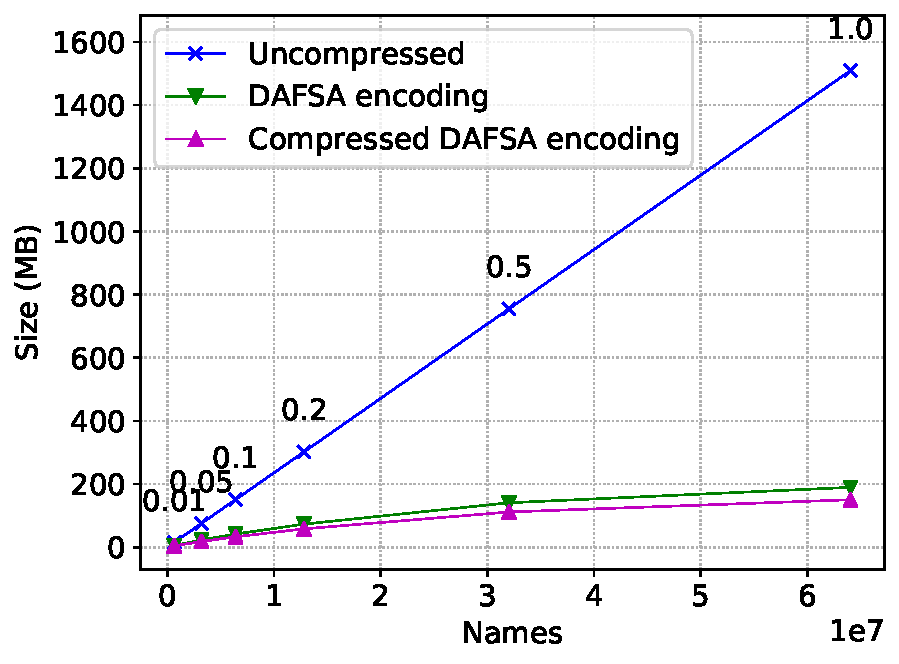
\includegraphics[width=\linewidth]{fig/sample}
  \caption{Size of the signaling set in various representations when 
           the names in the set are subsampled from the full set of names. 
           The labels above each distinct value on the $x$-axis
           denote the fraction of the full set that was sampled.}
  \label{fig:sample}
\end{figure}

\autoref{fig:sample} shows the results. If the fraction of domains that use
multiple independent certificate chains for the same name is small, as we would
anticipate, then \ac{name} clients significantly reduce their memory and disk
usage. For example, even if 10\% of all HTTPS websites deployed additional
certificates, the compressed DAFSA representation would require just under
33~MB. Of course, at very low levels of adoption, the advantage of the
\ac{dafsa}-based approach over a list of names decreases. This makes sense,
given that the \ac{dafsa} takes advantage of common substrings (especially
prefixes and suffixes) in a set.

\subsection{Signaling Set Updates}
\label{sec:evaluation:updates}

%\begin{figure*}[t]
  %\centering
  %\subfloat[Size of different representations of added names over time.]{
    %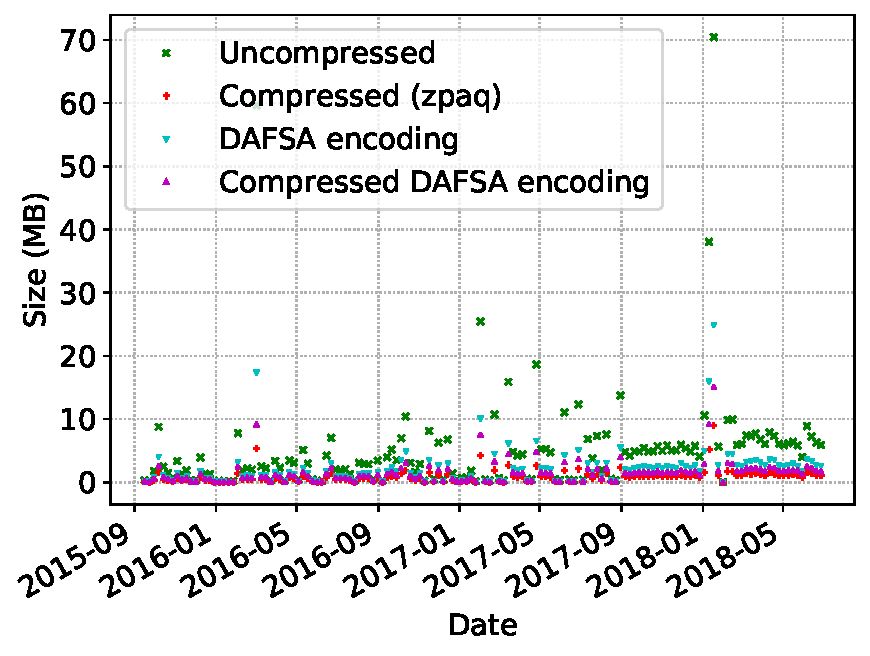
\includegraphics[width=0.5\linewidth]{fig/added_name_set_size}
    %\label{fig:updates:added}
  %}
  %\subfloat[Size of different representations of deleted names over time.]{
    %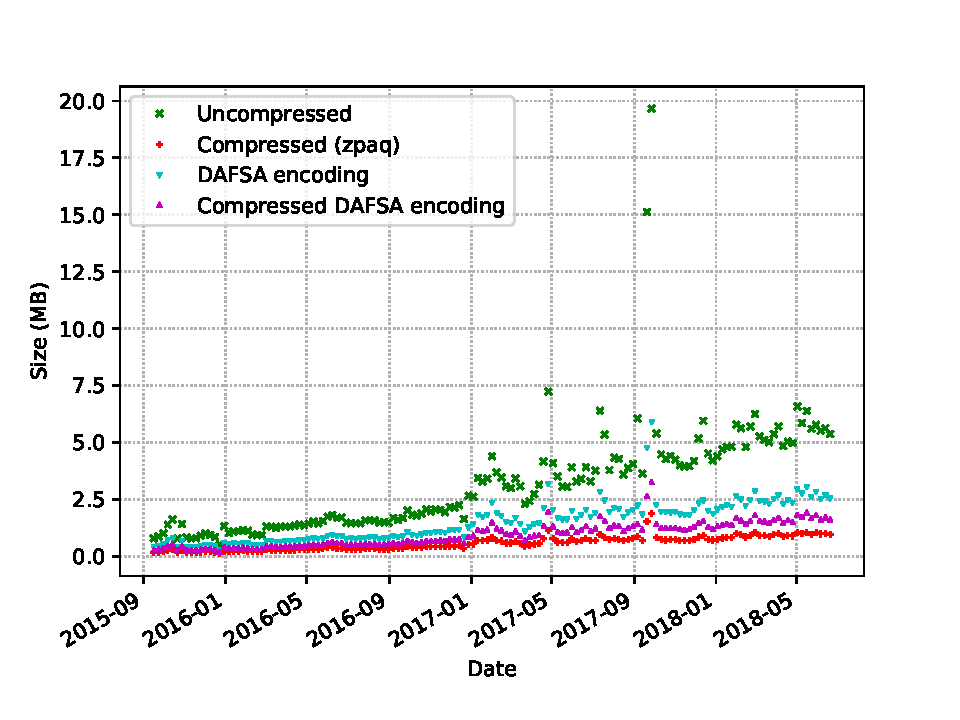
\includegraphics[width=0.5\linewidth]{fig/deleted_name_set_size}
    %\label{fig:updates:deleted}
  %}
  %\caption{Size of update sets over time.}
  %\label{fig:updates}
%\end{figure*}

\begin{figure}[t]
  \centering
  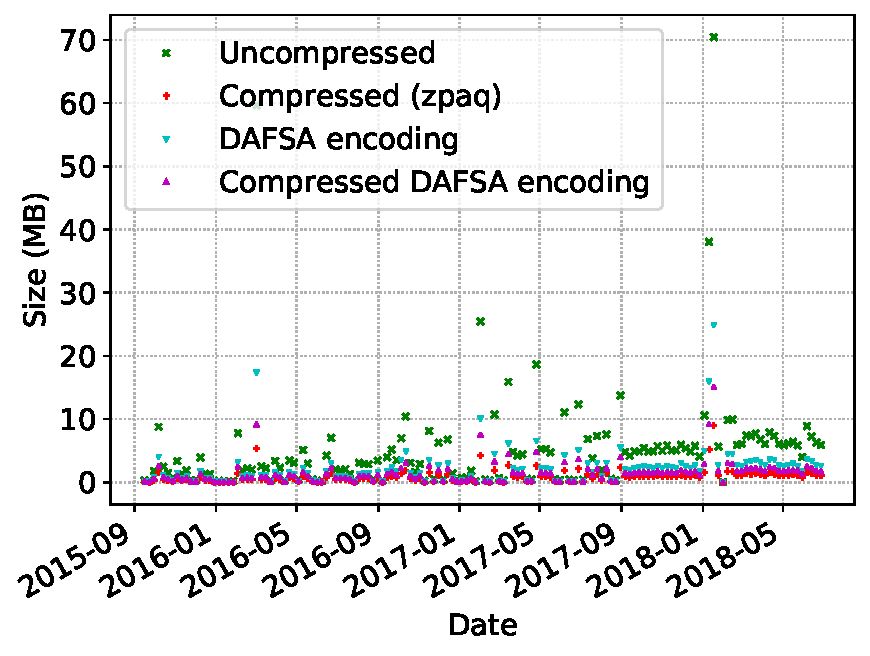
\includegraphics[width=\linewidth]{fig/added_name_set_size}
  \caption{Size of added name sets over time.}
  \label{fig:updates:added}
\end{figure}

Because the signaling set will be updated over time, we also carried out an
experiment to determine the size of updates that will be sent to clients. 
An update to the signaling set consists of the names added to the signaling
set since the most recent version, as well the names 
deleted due to certificate expiration or revocation. We computed the set of
added and deleted names for our range of scans, aggregating these sets by week.
We then computed the sizes of these sets in four different representations:
\begin{inparaenum}[(1)]
\item as an uncompressed text file of name strings,
\item as a compressed zpaq archive containing the above file,
\item as \iac{dafsa} of the set of strings, and
\item as a compressed zpaq archive containing the above \ac{dafsa}.
\end{inparaenum}
For each method, we used the variant that produced the smallest representation;
for example, we used the zpaq method that produced the smallest archive (method
5 with 64 MiB blocks) and our \ac{dafsa} representation used path compaction.
We experimented with the full set of names.

Figures~\ref{fig:updates:added} and~\ref{fig:updates:deleted} show the
results. As Figures~\ref{fig:count:certs} and~\ref{fig:count:names} would
indicate, the size of the signaling set has increased over time, and thus the
set of added names is consistently larger than the set of deleted names. Given
the relatively modest sizes of these sets compared to that of the full signaling
set, the most space-efficient method for representing and transmitting these
updates to clients is a zpaq-compressed archive of the raw text file of names
rather than \iac{dafsa}-based representation. From a technical perspective, this
method of transmission is also advantageous: clients can simply add the set of
added names to their existing \ac{dafsa}, and build (and subsequently add to) a
new \ac{dafsa} for the set of deleted names. Our results show that updates
(added and deleted names) are typically less than 3~MB per week or
$\sim$439~KB/day; by comparison, downloading the Google homepage requires
approximately 400~KB.

% BP: Why release once a week instead of every day?
%Releasing signaling set updates each week means that some false positives and
%false negatives are possible in \ac{name}, albeit under limited circumstances.
%Specifically, false positives (which render a domain inaccessible) are possible
%for up to a week, but only if a domain chooses to no longer serve its site over
%\ac{https}, lets its certificates expire, and does not inform the log
%aggregators in advance. False negatives (which enable \ac{tls} stripping
%attacks) are possible for up to a week, but only if a domain newly deploys
%\ac{https} by having a certificate issued and then immediately begins serving
%its site. Thus, not only are these pitfalls unlikely in practice, with advance
%planning and minimal effort, domains can avoid both of these situations.

% Put the figures here to make them display on a single page.
%\begin{figure}[t]
  %\centering
  %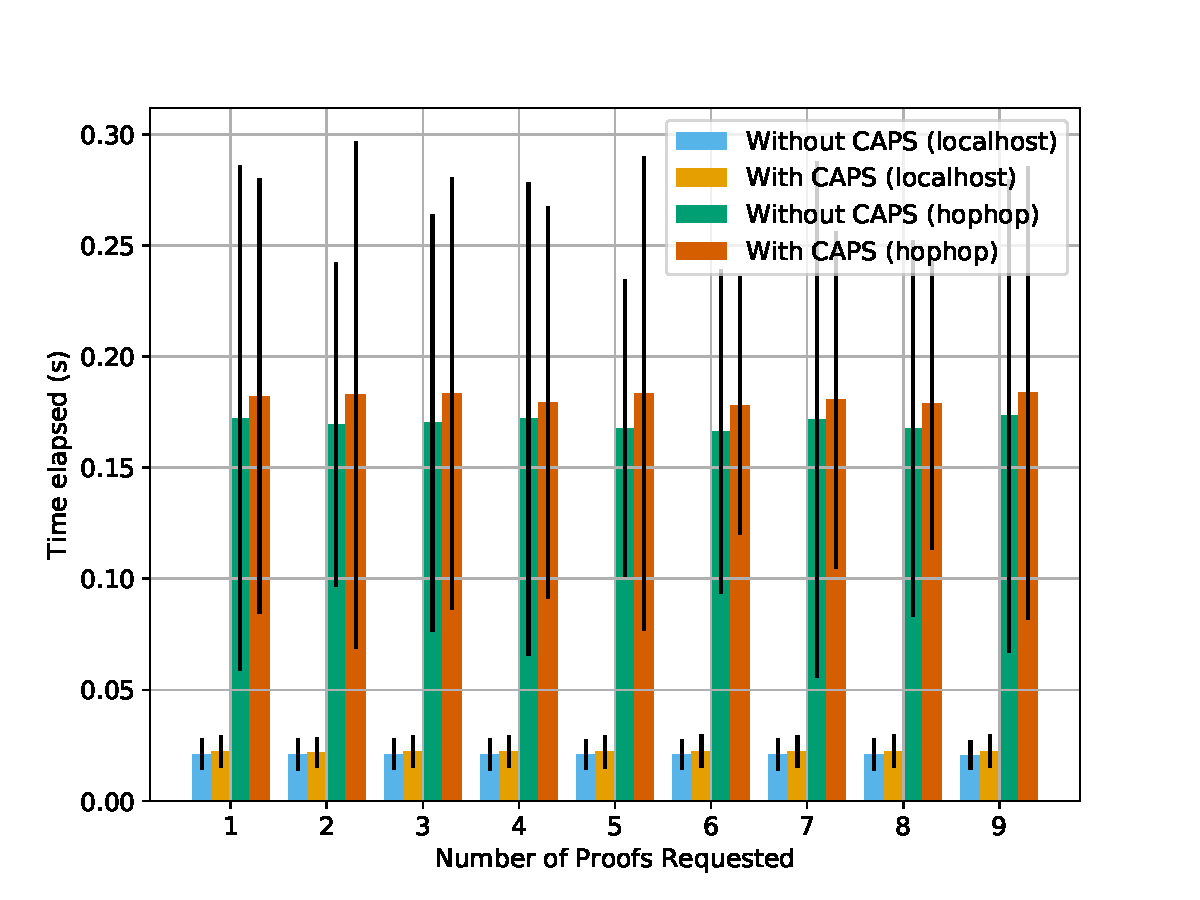
\includegraphics[width=\linewidth]{fig/eval_tls_ext/0-time_elapsed_vs_num_proofs_requested}
  %\caption{Handshake latency with different numbers of proofs requested. Error
  %bars represent standard error.}
  %\label{fig:evaltlsext:numproof}
%\end{figure}

%\begin{figure}[t]
  %\centering
  %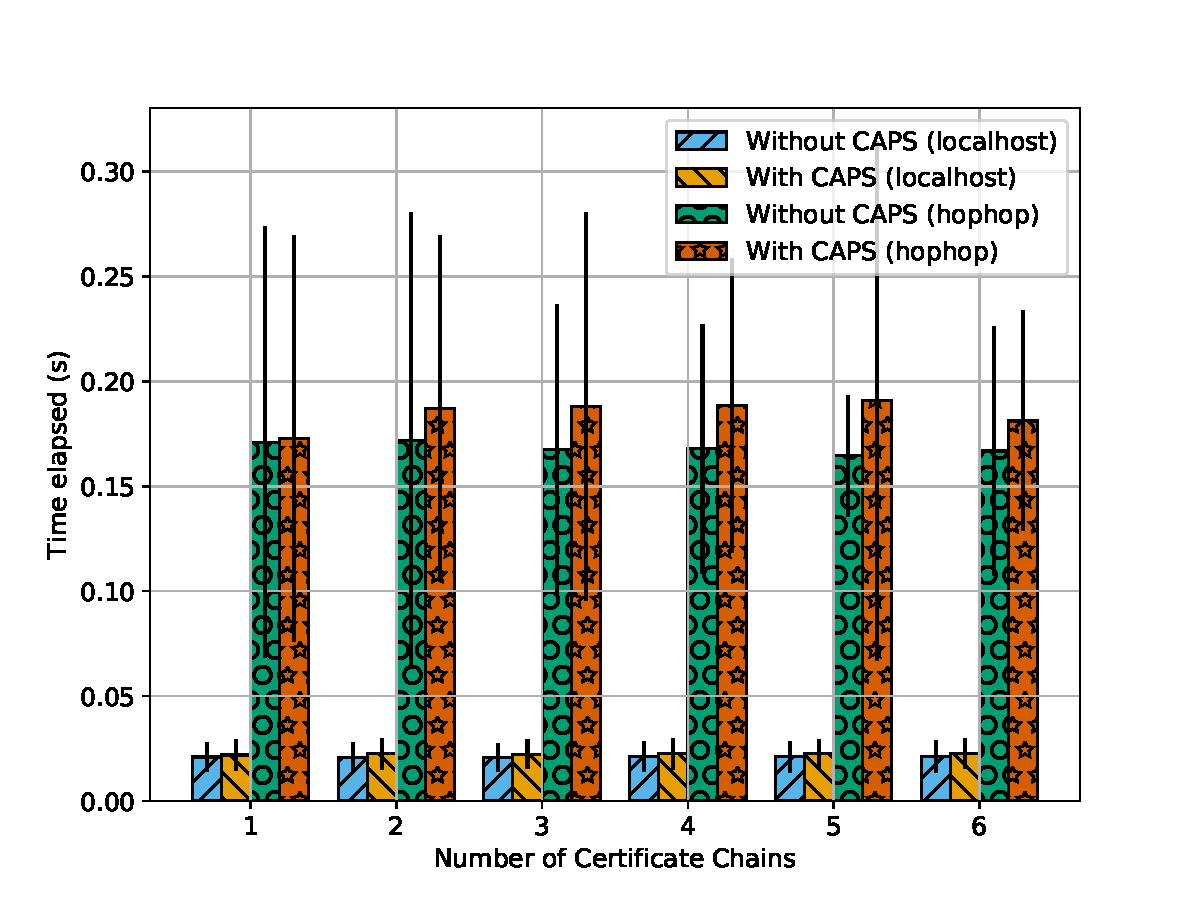
\includegraphics[width=\linewidth]{fig/eval_tls_ext/1-time_elapsed_vs_num_chains_sent}
  %\caption{Handshake latency with different numbers of certificate chains sent
  %from the server. Error bars represent standard error.}
  %\label{fig:evaltlsext:numchain}
%\end{figure}

%\begin{figure}[t]
  %\centering
  %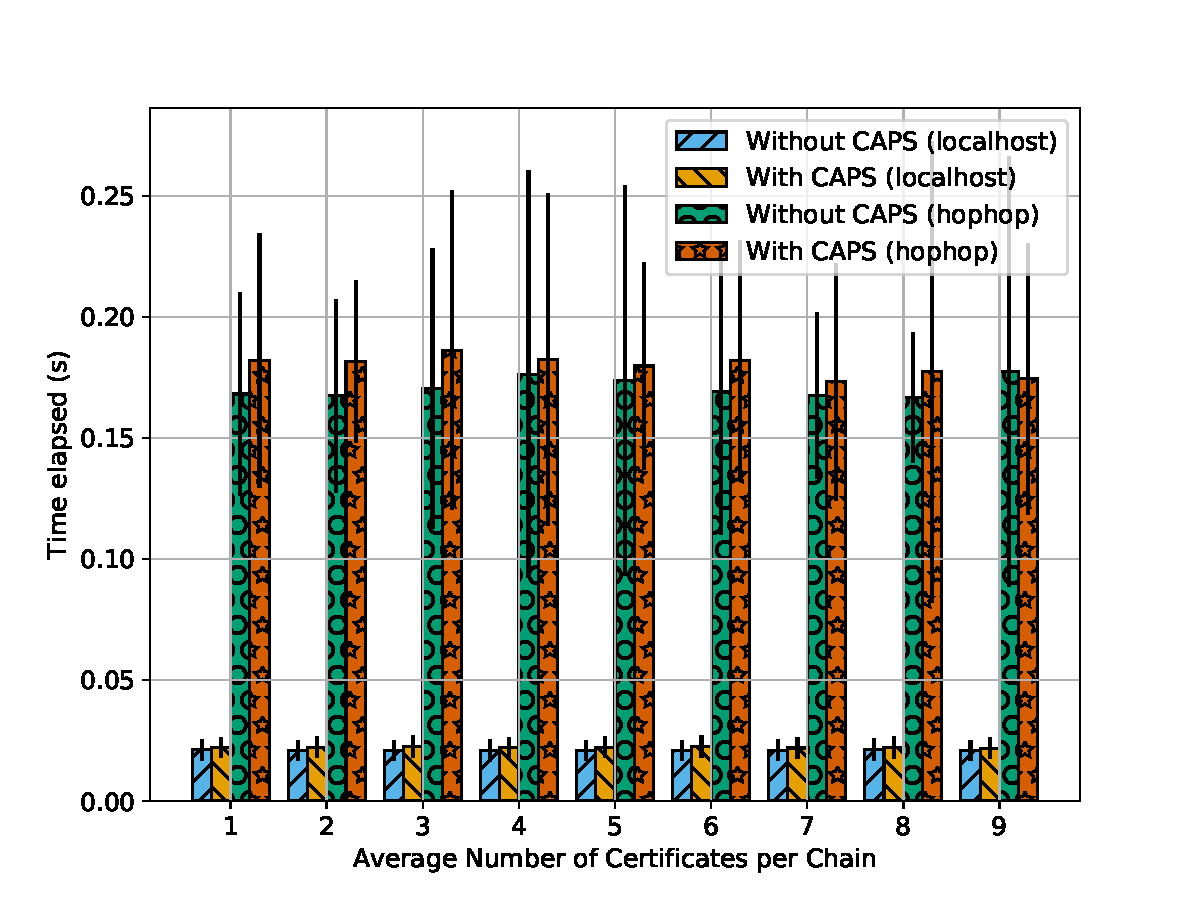
\includegraphics[width=\linewidth]{fig/eval_tls_ext/2-time_elapsed_vs_num_certs_per_chain}
  %\caption{Handshake latency with different average certificate chain length (in
  %certificates). Error bars represent standard error.}
  %\label{fig:evaltlsext:numcert}
%\end{figure}

%\begin{figure}[t]
  %\centering
  %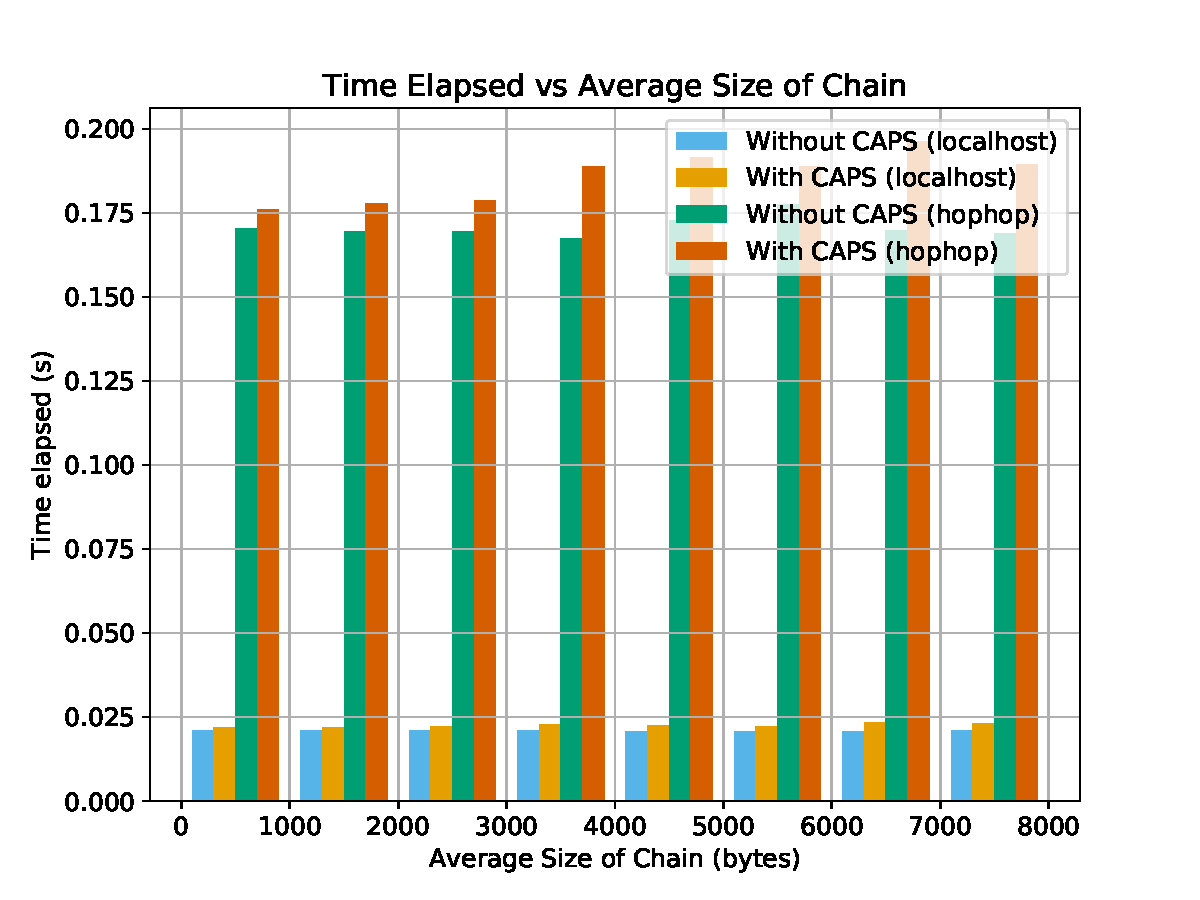
\includegraphics[width=\linewidth]{fig/eval_tls_ext/3-time_elapsed_vs_avg_chain_size}
  %\caption{Handshake latency with different average certificate chain size (in
  %bytes). Error bars represent standard error.}
  %\label{fig:evaltlsext:sizechain}
%\end{figure}

\subsection{Connection Establishment}
\label{sec:evaluation:performance}

\begin{figure*}[thb]
  \centering
  \subfloat[Proof count]{
    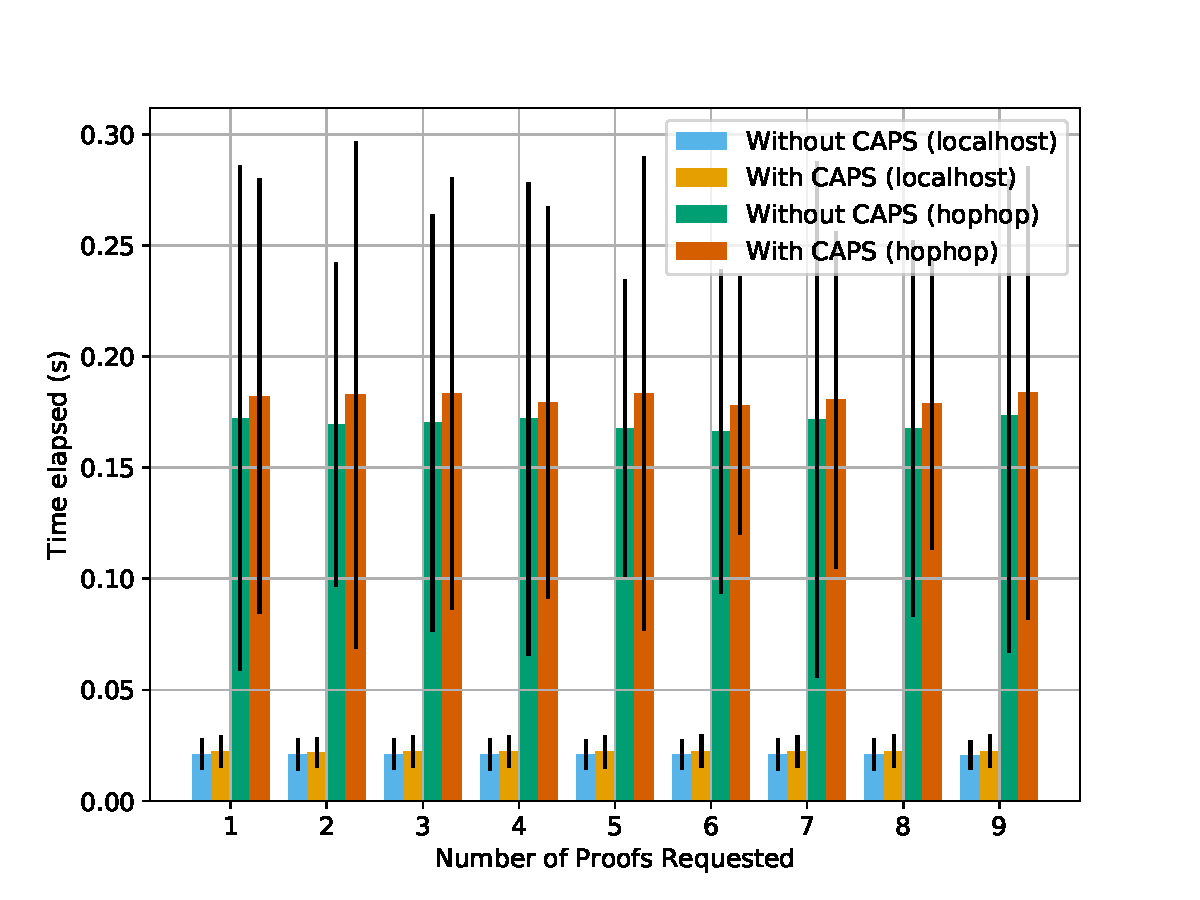
\includegraphics[width=0.5\linewidth]{fig/eval_tls_ext/0-time_elapsed_vs_num_proofs_requested}
    \label{fig:evaltlsext:numproof}
  }
  \subfloat[Chain count]{
    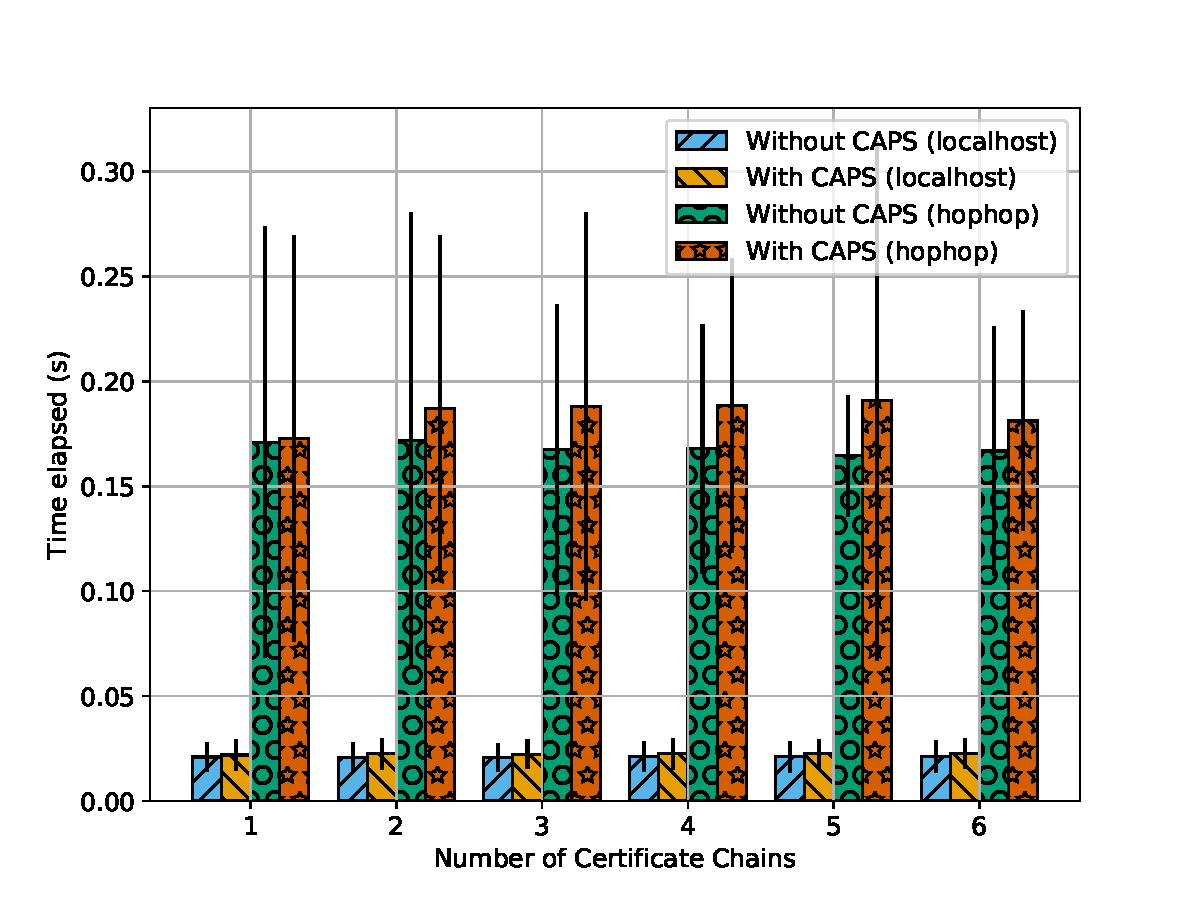
\includegraphics[width=0.5\linewidth]{fig/eval_tls_ext/1-time_elapsed_vs_num_chains_sent}
    \label{fig:evaltlsext:numchain}
  }
  \caption{Handshake latency in different scenarios. Error bars represent
  standard error.}
  \label{fig:evaltlsext}
\end{figure*}
To measure the performance of connection establishment in \ac{name}, we
implemented the handshake as a custom \ac{tls} extension in the OpenSSL library.
For concrete evaluation of this extension, we use \texttt{nginx} and \texttt{curl} with minor
modifications to use our \ac{tls} extension.

Additionally, we constructed sample sets of domain names based on four parameters:
\begin{inparaenum}
\item the number of proofs requested by the client during the
  ClientHello message (\numlas),
\item the number of certificate chains the domain sends during the ServerHello
  message (\policy),
\item the average number of certificates per chain, and
\item the average size of each certificate chain.
\end{inparaenum}
While varying each of these parameters, we measured the amount of extra data
sent in the \ac{name} handshake, and the latency of the handshake both with and
without the \ac{name} \ac{tls} extension.

We tested this both over the Internet (by connecting to a virtual private server
with latency varying from 30 to 300 ms), as well
as over the local loopback interface. The
tests over the internet (\emph{WAN}) provide an indication of the effect of
the extension on ``real world'' servers, 
whereas the \emph{localhost} tests provide a lower bound on time added due to
sending/receiving/processing extra data. A total of 15385 TLS connections were
established for our testing: 5768 over WAN, 9617 over localhost.

Our results in Figures~\ref{fig:evaltlsext:numproof},
\ref{fig:evaltlsext:numchain}, \ref{fig:evaltlsext:numcert}, and
\ref{fig:evaltlsext:sizechain} show that in comparison to the mean time
elapsed, there is an approximately 5\% increase in connection establishment
time: an average of 11ms longer for WAN and 1.2ms for localhost. 
Since our \ac{tls} extension does not add any extra round-trips to the
handshake, the time added is small, especially in comparison to random
measurement fluctuations (e.g., when we look at confidence intervals within one
standard deviation from the mean --- shown as error bars in the figures).

The extra data sent in the \ac{name} handshake is directly dependent on the size
and number of certificate chains, as well as the number of proofs sent. In
particular, the extra data sent from client to server is 1 byte, and the extra
data sent from server to client is
$(2 + (292 \times \text{\#proofs}) +
(\sum_{\text{chain}}\texttt{sizeof}(\text{chain})))$ bytes. 
%While this means
%that some connections may result in a great deal of extra data sent, we can
%expect that the vast majority of domains will not send additional certificate
%chains and the overhead will remain small.
